\documentclass[a4paper]{article}

\usepackage{Sweave} %--------------------------------!
\usepackage{amsmath}
\usepackage{amssymb}
\usepackage{amsthm}
\usepackage{fancyhdr}
\usepackage[usenames, dvipsnames]{color}
\usepackage{verbatim}

\oddsidemargin 0cm
\topmargin -2.4cm     %I recommend adding these three lines to increase the
\textwidth 16.5cm   %amount of usable space on the page (and save trees)
\textheight 27.5cm

\newcommand{\question}[2] {\vspace{.25in} \hrule\vspace{0.5em}
\noindent{\bf #1: #2} \vspace{0.5em}
\hrule \vspace{.10in}}
\renewcommand{\part}[1] {\vspace{.10in} {\bf (#1)}}

\newcommand{\myname}{Xuan Han}
\newcommand{\myhusky}{han.xua@husky.neu}
\newcommand{\myhwnum}{7}

\setlength{\parindent}{0pt}
\setlength{\parskip}{5pt plus 1pt}

\pagestyle{fancyplain}
\lhead{\fancyplain{}{\textbf{HW\myhwnum}}}      % Note the different brackets!
\rhead{\fancyplain{}{\myname\\ \myhusky}}
\chead{\fancyplain{}{1 2 3}}


\begin{document}
\Sconcordance{concordance:pca.tex:pca.Rnw:%
1 45 1 1 2 4 0 1 2 1 1 1 2 1 0 1 1 13 0 1 5 3 0 1 2 6 1 4 0 1 2 7 1 1 2 %
1 0 1 1 9 0 1 2 6 1 4 0 1 2 7 1 1 2 1 0 1 1 13 0 1 2 6 1 4 0 2 2 1 0 1 %
1 9 0 1 2 6 1 4 0 1 2 21 1 1 2 5 0 1 3 5 0 1 2 8 1 1 2 5 0 1 2 24 1 1 2 %
1 0 1 1 7 0 1 2 1 1 1 2 1 0 1 1 7 0 1 2 13 1}


\title{Data Mining Assignment \myhwnum}
\author{\myname \\
        \myhusky}
\date{\today}
\maketitle

\thispagestyle{plain}


\question{1}{PCA}
\begin{Schunk}
\begin{Sinput}
> load('hw7.RData')
\end{Sinput}
\end{Schunk}

\part{a}
\begin{Schunk}
\begin{Sinput}
> pr.out = prcomp(t(countsTableFull), scale. = FALSE)
> summary(pr.out)
\end{Sinput}
\begin{Soutput}
Importance of components:
                             PC1       PC2       PC3       PC4       PC5
Standard deviation     7.025e+05 4.001e+05 2.080e+05 1.437e+05 1.013e+05
Proportion of Variance 6.781e-01 2.200e-01 5.943e-02 2.839e-02 1.410e-02
Cumulative Proportion  6.781e-01 8.981e-01 9.575e-01 9.859e-01 1.000e+00
                             PC6
Standard deviation     9.594e-10
Proportion of Variance 0.000e+00
Cumulative Proportion  1.000e+00
\end{Soutput}
\begin{Sinput}
> Cols = function(vec) {
+     cols = rainbow(length(vec))
+     return (cols[as.numeric(as.factor(vec))])
+ }
> par(mfrow = c(2, 2))
> labs = c('N','N','N', 'T','T','T')
> plot(pr.out$x[, 1:2], col = Cols(labs), pch = 19, xlab = 'Z1', ylab = 'Z2')
> plot(pr.out)
> pve = 100 * pr.out$sdev ^ 2 / sum(pr.out$sdev ^ 2)
> plot(pve, type = 'o', ylab = 'PVE', xlab = 'Principle Component', col = 'blue')
> plot(cumsum(pve), type = 'o', ylab = 'Cumulative PVE', xlab = 'Principle Component', col = 'red')
\end{Sinput}
\end{Schunk}
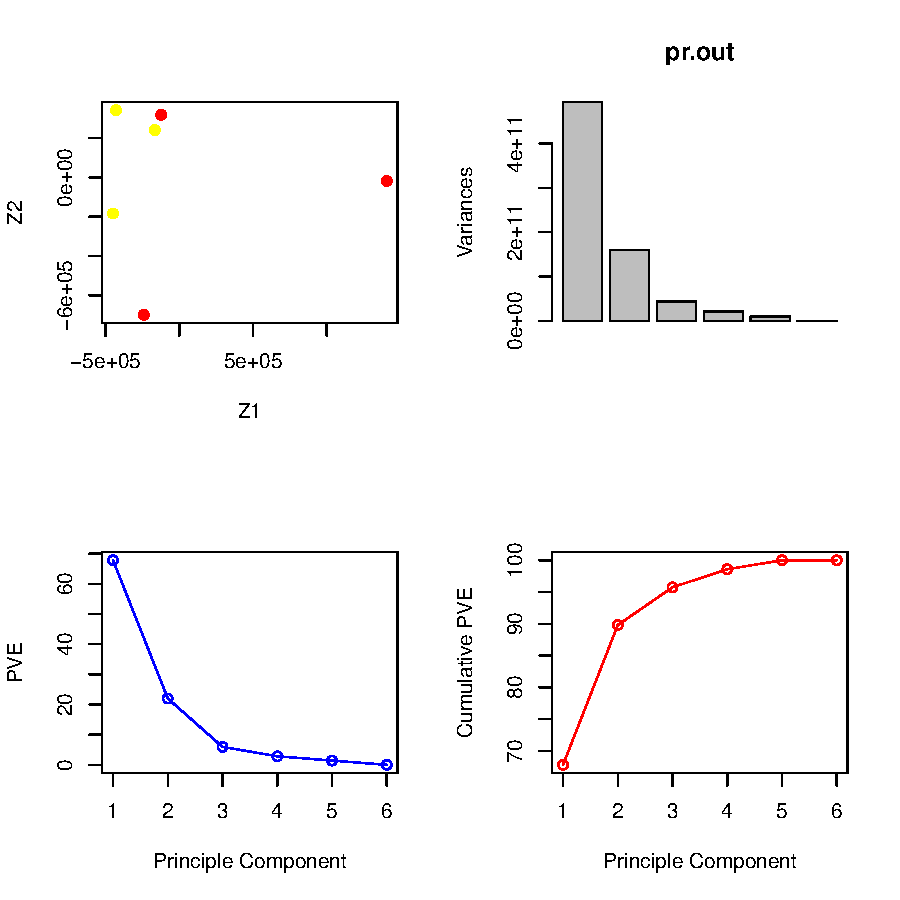
\includegraphics{pca-1a}
\begin{enumerate}
{\color{red}
\item There are 6 components in this dataset. Because there are min(p, n) components in general. In this case, p = 10453, n = 6.
\item A desirable score plot will be able to seperate the two different type of tissues. The score plot shows a desirable plot, but not so good.
}
\end{enumerate}

\part{b}
\begin{Schunk}
\begin{Sinput}
> pr.out2 = prcomp(t(countsTableFull), scale. = TRUE)
> summary(pr.out2)
\end{Sinput}
\begin{Soutput}
Importance of components:
                           PC1     PC2     PC3      PC4      PC5       PC6
Standard deviation     76.7068 43.8169 34.4531 32.09464 20.78593 9.907e-14
Proportion of Variance  0.5629  0.1837  0.1136  0.09854  0.04133 0.000e+00
Cumulative Proportion   0.5629  0.7466  0.8601  0.95867  1.00000 1.000e+00
\end{Soutput}
\begin{Sinput}
> par(mfrow = c(2, 2))
> labs = c('N','N','N', 'T','T','T')
> plot(pr.out2$x[, 1:2], col = Cols(labs), pch = 19, xlab = 'Z1', ylab = 'Z2')
> plot(pr.out2)
> pve = 100 * pr.out2$sdev ^ 2 / sum(pr.out2$sdev ^ 2)
> plot(pve, type = 'o', ylab = 'PVE', xlab = 'Principle Component', col = 'blue')
> plot(cumsum(pve), type = 'o', ylab = 'Cumulative PVE', xlab = 'Principle Component', col = 'red')
\end{Sinput}
\end{Schunk}
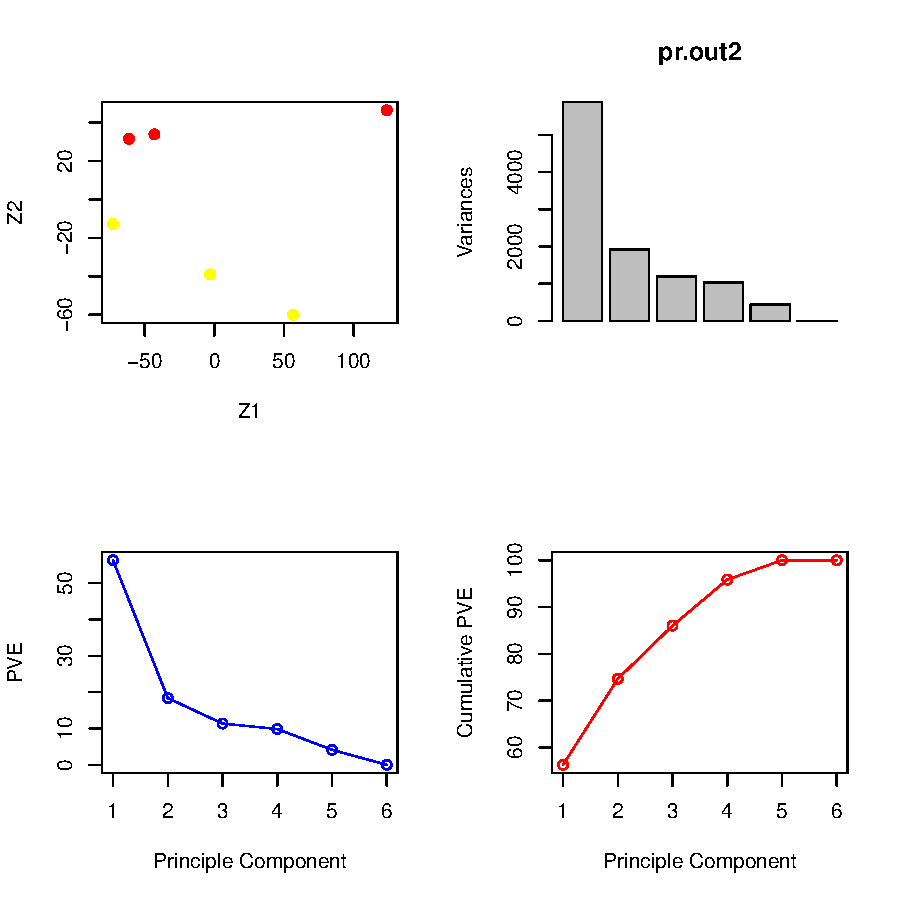
\includegraphics{pca-1b}
\begin{enumerate}
{\color{red}
\item Obviously the two tissues seperated more clearly, which is a desirable result.
\item The PVE of the first two priciple components decreased.
}
\end{enumerate}

\part{c}
\begin{Schunk}
\begin{Sinput}
> pr.out = prcomp(t(countsTableSubset), scale. = FALSE)
> summary(pr.out)
\end{Sinput}
\begin{Soutput}
Importance of components:
                             PC1       PC2       PC3       PC4      PC5
Standard deviation     4.815e+04 2.271e+04 9.040e+03 5.141e+03 4.53e+03
Proportion of Variance 7.825e-01 1.741e-01 2.758e-02 8.920e-03 6.93e-03
Cumulative Proportion  7.825e-01 9.566e-01 9.841e-01 9.931e-01 1.00e+00
                             PC6
Standard deviation     1.172e-11
Proportion of Variance 0.000e+00
Cumulative Proportion  1.000e+00
\end{Soutput}
\begin{Sinput}
> par(mfrow = c(2, 2))
> labs = c('N','N','N', 'T','T','T')
> plot(pr.out$x[, 1:2], col = Cols(labs), pch = 19, xlab = 'Z1', ylab = 'Z2')
> plot(pr.out)
> pve = 100 * pr.out$sdev ^ 2 / sum(pr.out$sdev ^ 2)
> plot(pve, type = 'o', ylab = 'PVE', xlab = 'Principle Component', col = 'blue')
> plot(cumsum(pve), type = 'o', ylab = 'Cumulative PVE', xlab = 'Principle Component', col = 'red')
\end{Sinput}
\end{Schunk}
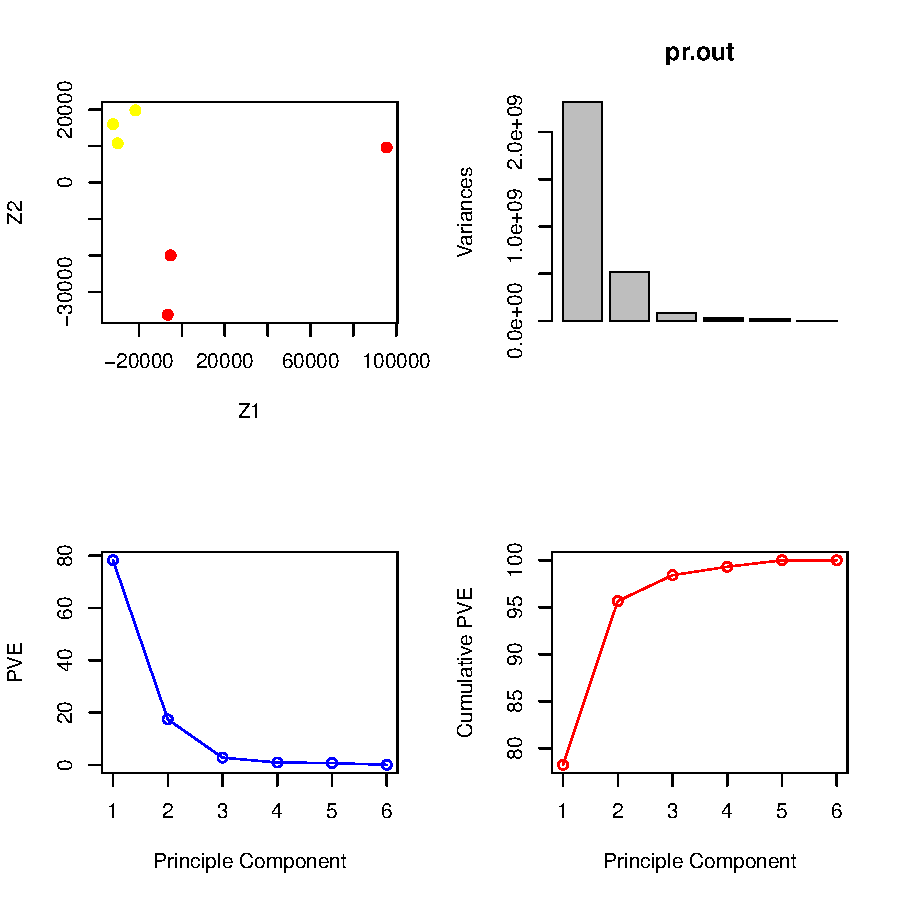
\includegraphics{pca-1c}

\begin{Schunk}
\begin{Sinput}
> pr.out2 = prcomp(t(countsTableSubset), scale. = TRUE)
> summary(pr.out2)
\end{Sinput}
\begin{Soutput}
Importance of components:
                           PC1    PC2     PC3    PC4     PC5       PC6
Standard deviation     17.7897 8.6068 4.17155 3.4163 3.06252 4.401e-15
Proportion of Variance  0.7377 0.1727 0.04056 0.0272 0.02186 0.000e+00
Cumulative Proportion   0.7377 0.9104 0.95093 0.9781 1.00000 1.000e+00
\end{Soutput}
\begin{Sinput}
> par(mfrow = c(2, 2))
> labs = c('N','N','N', 'T','T','T')
> plot(pr.out2$x[, 1:2], col = Cols(labs), pch = 19, xlab = 'Z1', ylab = 'Z2')
> plot(pr.out2)
> pve = 100 * pr.out2$sdev ^ 2 / sum(pr.out2$sdev ^ 2)
> plot(pve, type = 'o', ylab = 'PVE', xlab = 'Principle Component', col = 'blue')
> plot(cumsum(pve), type = 'o', ylab = 'Cumulative PVE', xlab = 'Principle Component', col = 'red')
\end{Sinput}
\end{Schunk}
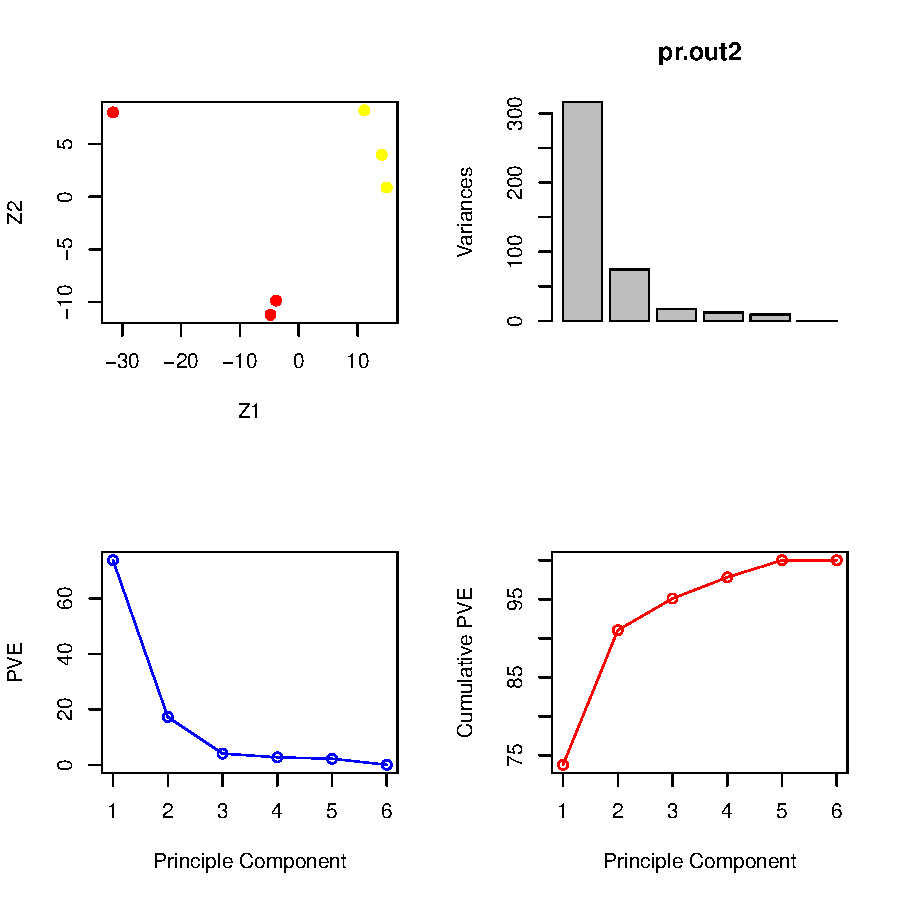
\includegraphics{pca-1c2}

\begin{enumerate}
{\color{red}
\item We can find simmilar result with this data set, such as the PVE of first two components decrease after scaling.
\item And the two type of tissues seperated more clearly after scaling.
}
\end{enumerate}

\part{d}
{\color{red}
Suggestions:\\
\begin{enumerate}
\item Scale the variables before do clustering.
\item Use at leart first 3 principle components to do analysis.
\end{enumerate}
}


\newpage
\question{2}{Clustering and headmaps}

\part{a}
\begin{Schunk}
\begin{Sinput}
> heatmap(t(countsTableSubset), scale = 'none')
\end{Sinput}
\end{Schunk}
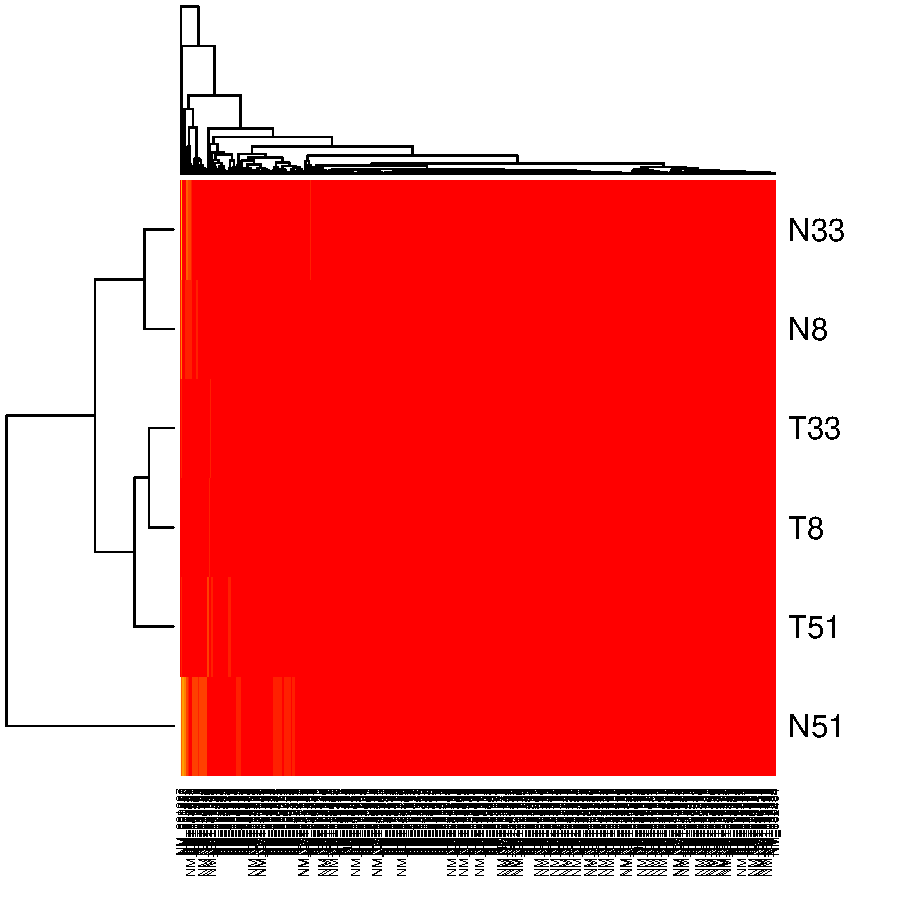
\includegraphics{pca-2a2}
\begin{Schunk}
\begin{Sinput}
> heatmap(t(countsTableSubset), scale = 'col')
\end{Sinput}
\end{Schunk}
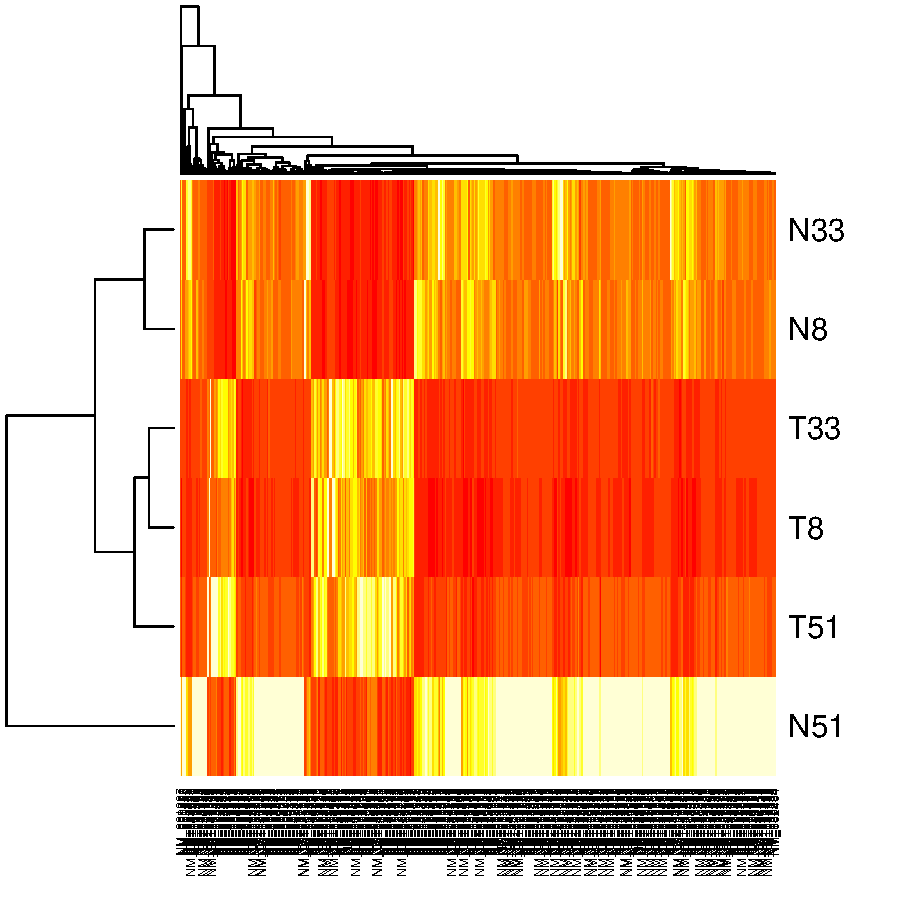
\includegraphics{pca-2a}
{\color{red}
\begin{enumerate}
\item Obviouly there is a big difference before and after scale.
\item Scaling has no effect on the apperance of the dendrograms. Because scaling is done after dendrograms is calculated.
\item Scaling has a big effect on the apperance of the heat map. Scaling make things on different scale comparable and thus easier to see the difference.
\end{enumerate}
}

\part{b}
\begin{Schunk}
\begin{Sinput}
> heatmap(t(countsTableSubset), scale = 'col', distfun = function(x) as.dist((1 - cor(t(x)))))
\end{Sinput}
\end{Schunk}
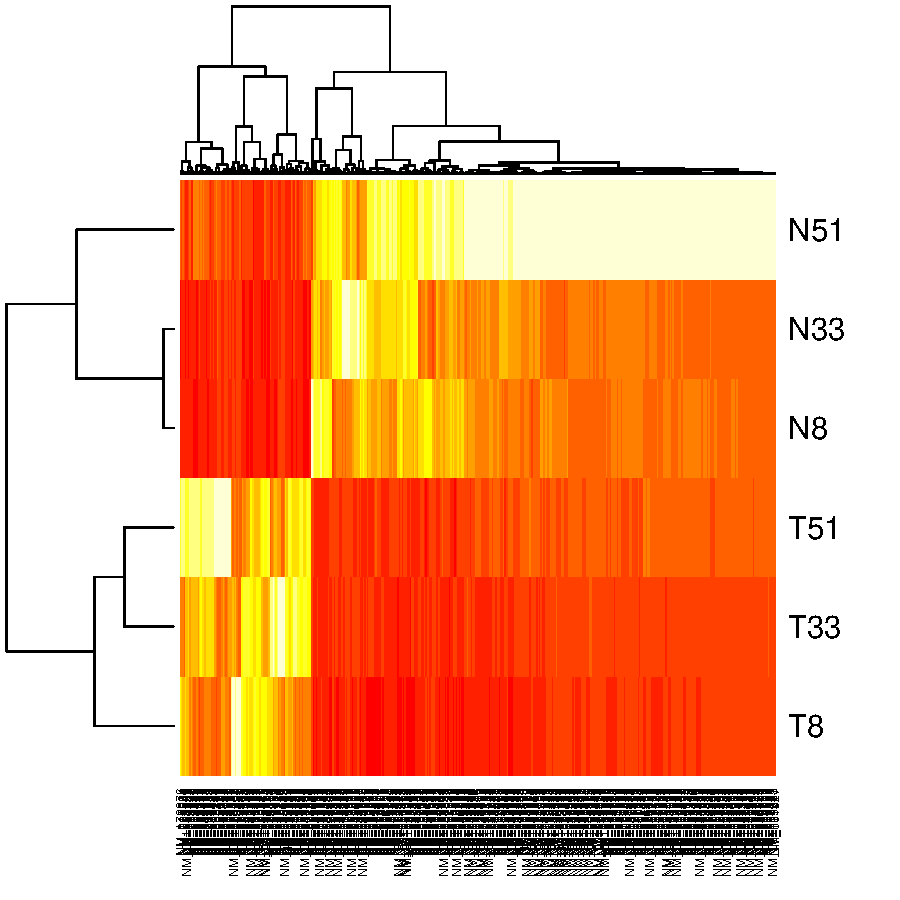
\includegraphics{pca-2b}
{\color{red}
\begin{enumerate}
\item Similarity: In both cases, cluster assignment of T8, T33, T51, N8, N33 are similar.
\item Difference: By using Corrleation distance, we find that cluster assignment of N51 changed. Corrleation tend to do a better job, since it assigned N51 to the right cluster.
\item Because Corrleation distance pay more attention to the pattern of the feature vectors , and pay less attention to magnitude of feature vectors. But Eucledian distance do in the opposite way.
\end{enumerate}
}

\part{c}
{\color{red}
Summary:
\begin{enumerate}
\item We find obvious difference between scaling and not scaling.
\item We have different result using Eucledian distance and Corrleation distance. The latter is better.
\end{enumerate}
Suggestions:
\begin{enumerate}
\item Scale before plot headmap.
\item First, Try different distance to see different result. And then select the best distance. For this specific case, use Corrleation distance.
\end{enumerate}
}

\newpage
\question{3}{Kmeans}
\part{a}
\begin{Schunk}
\begin{Sinput}
> km.out = kmeans(t(countsTableFull), 2, nstart = 50)
> km.out$cluster
\end{Sinput}
\begin{Soutput}
 N8 N33 N51  T8 T33 T51 
  1   1   2   1   1   1 
\end{Soutput}
\end{Schunk}

\part{b}
\begin{Schunk}
\begin{Sinput}
> km.out = kmeans(t(countsTableSubset), 2, nstart = 50)
> km.out$cluster
\end{Sinput}
\begin{Soutput}
 N8 N33 N51  T8 T33 T51 
  2   2   1   2   2   2 
\end{Soutput}
\end{Schunk}

{\color{red}
In both cases, N51 is assigned to one cluster, and all others are assigned to one cluster. The result is very poor.
}

\part{c}
{\color{red}
Suggestions:
\begin{enumerate}
\item For future analysis of such data, it's better to use hierarchical clustering.
\end{enumerate}
}

\end{document}
